\chapter{Primera ley de la termodinámica}

\section{Calor y trabajo termodinámico}

\subsection*{Definición cuantitativa del calor}

Ya que las diferencias de energía entre dos estados de equilibrio son medibles, es posible usar
este hecho para definir cuantitativamente el calor:

\begin{definicion}[Calor]
  El flujo de calor de un sistema en un proceso dado (a un número de moles constante) es
  simplemente la diferencia de la energía interna entre los estados inicial y final menos el
  trabajo realizado en este proceso.
\end{definicion}

Consideremos un proceso que lleva a un sistema del estado $A$ al estado $B$. ¿Cómo sabemos cuál
es la cantidad de energía transferida al sistema en forma de trabajo y cuánta en forma de calor
para dicho proceso?
\begin{itemize}[itemsep=0pt]
  \item Trabajo: métodos mecánicos.
  \item Energía: $U_B-U_A$ (sistema adiabático).
\end{itemize}

Asumamos que existen diferentes procesos que llevan al sistema del estado $A$ al estado $B$ (es
decir, independientemente del proceso, el sistema pasa siempre de $A\to B$).
\begin{figure}[H]
  \centering
  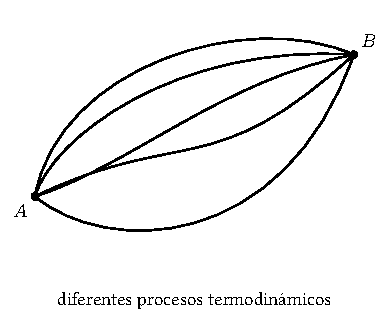
\includegraphics{figuras/procesos-AB.pdf}
\end{figure}
Para cada uno de estos procesos la cantidad de trabajo realizado puede variar; lo mismo ocurre con
el flujo de calor, pero $\Delta U=U_B-U_A$ es siempre la misma independientemente del proceso.
Por lo tanto, $\Delta U$ queda determinada por los estados inicial y final, mientras que el flujo
de calor y el trabajo realizado \textbf{sí} dependen del proceso considerado.

\subsubsection*{Trabajo cuasiestático}

Restringiendo por el momento la atención hacia sistemas termodinámicos simples (de carácter
hidrostático), podemos decir que el \textbf{trabajo cuasiestático} asociado con un cambio de
volumen está dado cuantitativamente por
\begin{equation*}
  \dbar W=-P\,\dd V,
\end{equation*}
donde $P$ es la presión. % NOTA (manuscrito): "¿Por qué este símbolo?" sobre la barra en $\dbar$ (diferencial inexacta).
Esta relación solo es válida para los llamados procesos cuasiestáticos.

\begin{definicion}[Proceso cuasiestático]
  Un proceso cuasiestático es un proceso que ocurre tan lentamente que el sistema permanece en
  equilibrio en cualquier instante de tiempo.
\end{definicion}

\begin{figure}[H]
  \centering
  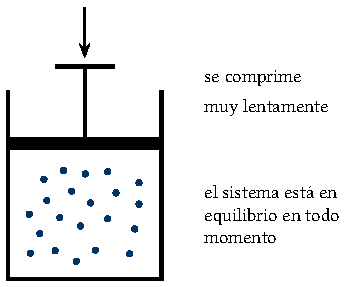
\includegraphics{figuras/cuasiestatico.pdf}
\end{figure}

\begin{observacion}
  \emph{¿Por qué $-P\,\dd V$?} La convención del signo del trabajo es considerar que este será positivo si incrementa la
  energía del sistema. Si el volumen del sistema disminuye, se hace trabajo \emph{sobre} el
  sistema, incrementando su energía; por lo tanto el signo es negativo. Así, $\dbar W=-P\,\dd V$
  (con $\dd V$ el cambio de volumen):
  \begin{itemize}[itemsep=0pt]
    \item si $\dd V>0$ (expansión), el sistema realiza trabajo positivo sobre el exterior (pierde
      energía);
    \item si $\dd V<0$ (compresión), el entorno (agente externo) realiza trabajo sobre el sistema y
      el trabajo del sistema es negativo (gana energía).
  \end{itemize}
  Esta perspectiva describe el trabajo realizado \emph{sobre} el sistema; es la más común en
  termodinámica.
\end{observacion}

La expresión anterior para el trabajo hidrostático permite dar una definición cuantitativa para el
calor. Sea un proceso cuasiestático infinitesimal (para un número de moles constante); entonces el
\textbf{calor cuasiestático} $\dbar Q$ (también denotado $\delta Q$) se define como
\begin{equation*}
  \dd U=\dbar Q+\dbar W\qquad(\text{para }N\text{ constante}),
\end{equation*}
es decir, los cambios en la energía interna son cambios en el calor más cambios en el trabajo.

\subsection*{Conservación de la energía y diferenciales inexactas}

¿Conservación de la energía? Sí. Equivalentemente, para un número de moles constante,
\begin{align*}
  \dbar Q&=\dd U-\dbar W,\\
  \dbar Q&=\dd U+P\,\dd V.
\end{align*}

El calor (o flujo de calor) representa solo otra forma de energía, como el trabajo; cuando la
energía es transferida a un sistema como trabajo o calor, es indistinguible de otras formas de
energía. Aunque $\dd U=\dbar Q+\dbar W$, esto \textbf{no} es equivalente a $U=Q+W$ para un estado
dado.

Por esta razón aparecen los símbolos $\dbar$ o $\delta$ para indicar que estos son
\textbf{diferenciales imperfectos} (o inexactos). En procesos infinitesimales, las integrales de
$\dbar Q$ y $\dbar W$ son el calor y el trabajo únicamente para dicho proceso, y su suma es
$\Delta U$, que siempre es independiente del proceso.

\begin{observacion}
  \emph{¿Por qué imperfectos?} Porque dependen del camino seguido para llegar de un estado a otro.
  Si bien sabemos que $\Delta U$ siempre es igual, $\dbar Q$ y $\dbar W$ pueden ser diferentes en
  cada trayectoria del diagrama $P$--$V$.
  \begin{figure}[H]
    \centering
    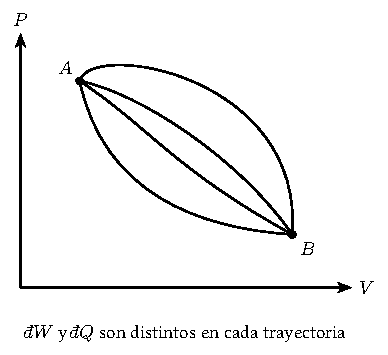
\includegraphics{figuras/PV-trayectorias.pdf}
  \end{figure}
\end{observacion}

\textbf{Unidades de energía.} Joule (MKS); $1\ \mathrm{erg}=1\times10^{-7}\ \mathrm{J}$ (cgs);
$1\ \mathrm{cal}=4.1858\ \mathrm{J}$.
% VERIFICAR: 1 cal = 4.1858 J (manuscrito; los valores usuales son 4.184 J o 4.1868 J).

\begin{ejemplo}
  Un gas dado está encerrado en un cilindro el cual tiene un pistón móvil. Si las paredes del
  cilindro son adiabáticas, se observa un incremento cuasiestático del volumen que resulta en una
  disminución de la presión de acuerdo con la siguiente ecuación:
  \begin{equation*}
    P^{3}V^{5}=\text{cte.}\qquad(\text{para }Q=0).
  \end{equation*}
  \begin{enumerate}[label=\alph*),itemsep=2pt]
    \item Encuentre el trabajo cuasiestático hecho sobre el sistema y la transferencia neta de calor
      al sistema en cada uno de los siguientes procesos: $ADB$, $ACB$ y el proceso directo $AB$
      mostrados en el diagrama $P$--$V$ presentado a continuación.
  \end{enumerate}
  \begin{figure}[H]
    \centering
    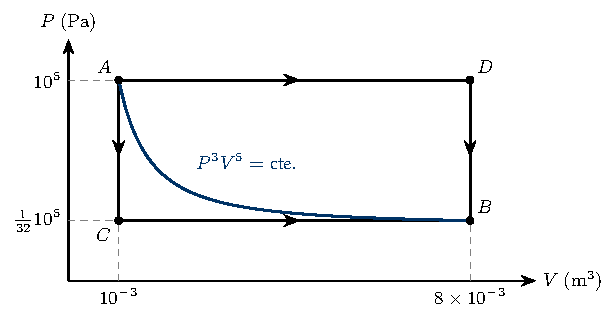
\includegraphics{figuras/PV-ejemplo.pdf}
  \end{figure}
  En el proceso $ADB$ el gas se calienta a presión constante ($P=10^{5}\,\mathrm{Pa}$) hasta que el
  volumen alcanza su valor final ($V=8\times10^{-3}\,\mathrm{m^3}$) [proceso $AD$]; posteriormente
  el gas se enfría, lo que disminuye la presión hasta $\tfrac{1}{32}\times10^{5}\,\mathrm{Pa}$. El
  resto de los procesos se puede interpretar similarmente.

  \emph{Nota:} una curva adiabática implica que, si existe un cambio en el volumen, debe ir seguido
  de un cambio en la presión para conservar la energía interna.
  % REVISAR (manuscrito): la nota dice "para conservar la energía interna"; en una adiabática Q=0 pero U sí cambia (aquí U_B-U_A=-112.5 J).

  \begin{solucion}
    Tenemos entonces que revisar cómo ocurre cada uno de los procesos.

    \textbf{Proceso $AB$.} Es una expansión adiabática, ya que el volumen aumenta pero disminuye la
    presión, sin cambios en el calor. Entonces $\dd U=\dbar Q^{\,0}+\dbar W$ para $AB$, es decir,
    $\dd U=-P\,\dd V$. Integrando,
    \begin{equation*}
      \int_{U_A}^{U_B}\dd U=-\int_{V_A}^{V_B}P\,\dd V
      \quad\Longrightarrow\quad
      U_B-U_A=-\int_{V_A}^{V_B}P\,\dd V.
    \end{equation*}
    Para resolver esta integral debemos retomar la relación $P^3V^5=\text{cte.}$; como esta
    cantidad siempre es constante, $P^3V^5=P_A^3V_A^5$ (o bien $P^3V^5=P_B^3V_B^5$), de donde
    \begin{equation*}
      P^3=P_A^3\left(\frac{V_A}{V}\right)^{\!5}
      \quad\Longrightarrow\quad
      P=\sqrt[3]{P_A^3\left(\frac{V_A}{V}\right)^{\!5}}=P_A\left(\frac{V_A}{V}\right)^{\!5/3}.
    \end{equation*}
    Así,
    \begin{align*}
      U_B-U_A&=-\int_{V_A}^{V_B}P_A\left(\frac{V_A}{V}\right)^{\!5/3}\dd V
        =-P_AV_A^{5/3}\int_{V_A}^{V_B}\frac{\dd V}{V^{5/3}}
        =-P_AV_A^{5/3}\left[\frac{1}{-\tfrac{2}{3}}\,V^{-2/3}\right]_{V_A}^{V_B}\\
      &=\frac{3}{2}\,P_AV_A^{5/3}\left(V_B^{-2/3}-V_A^{-2/3}\right)\\
      &=\frac{3}{2}\,(10^{5}\,\mathrm{Pa})(10^{-3}\,\mathrm{m^3})^{5/3}
        \Bigl[(8\times10^{-3}\,\mathrm{m^3})^{-2/3}-(10^{-3}\,\mathrm{m^3})^{-2/3}\Bigr]\\
      &=\frac{3}{2}\,(1\,\mathrm{N\,m^3})\Bigl[(25\,\mathrm{m^{-2}})-(100\,\mathrm{m^{-2}})\Bigr]
        =\frac{3}{2}\,(1\,\mathrm{N\,m^3})(-75\,\mathrm{m^{-2}}),
    \end{align*}
    donde se usó $[\mathrm{Pa}]=\mathrm{N/m^2}$ y $[\mathrm{m^3}]^{5/3}=\mathrm{m^5}$. Por lo tanto,
    \begin{equation*}
      \boxed{U_B-U_A=-112.5\ \mathrm{J}}
    \end{equation*}
    Este tipo de procesos son llamados procesos reversibles y se caracterizan por $\dbar Q=0$.

    \textbf{Proceso $ADB$.} En la parte $DB$ no hay cambio de volumen, por lo que
    $\dbar W=-P\,\dd V=0$; por lo cual solo en $AD$ se tiene $\dbar W\neq0$. Entonces
    \begin{align*}
      \Delta W_{ADB}&=-\int_{V_A}^{V_D}P\,\dd V=-P_A(V_D-V_A)\\
      &=-(1\times10^{5}\,\mathrm{Pa})(8\times10^{-3}\,\mathrm{m^3}-1\times10^{-3}\,\mathrm{m^3})\\
      &=-(1\times10^{5}\,\mathrm{Pa})(7\times10^{-3}\,\mathrm{m^3})\\
      \Delta W_{ADB}&=-700\ \mathrm{J}.
    \end{align*}
    Ahora, el proceso $ADB$ incluye un calentamiento para aumentar la presión y luego un
    enfriamiento, por lo que efectivamente $\Delta Q\neq0$, con $\dd U=\dbar Q+\dbar W$. Además,
    el punto inicial y final de los procesos $ADB$ y $AB$ es el mismo, por lo que
    $\Delta U_{ADB}=\Delta U_{AB}$. Luego
    \begin{align*}
      \Delta U_{AB}&=\Delta Q_{ADB}+\Delta W_{ADB}
        \quad\Longrightarrow\quad
        \Delta Q_{ADB}=\Delta U_{AB}-\Delta W_{ADB}\\
      \Delta Q_{ADB}&=-112.5\ \mathrm{J}-(-700\ \mathrm{J})=587.5\ \mathrm{J},
        \qquad\boxed{\Delta Q_{ADB}=587.5\ \mathrm{J}}
    \end{align*}
    En este caso particular se puede calcular $\Delta Q_{ADB}$, pero no $\Delta Q_{AD}$ o
    $\Delta Q_{DB}$ por separado, porque nos falta $\Delta U_{AD}$.

    \textbf{Proceso $ACB$.} El procedimiento es similar: ya que en $AC$, $\dd V=0$, para $AC$
    se tiene $\dbar W_{AC}=-P\,\dd V=0$, mientras que para $CB$ se tiene $\dbar W_{CB}=-P\,\dd V$, es
    decir,
    \begin{align*}
      \Delta W_{ACB}&=-\int_{V_C}^{V_B}P\,\dd V=-P_C(V_B-V_C)\\
      &=-\Bigl(\tfrac{1}{32}\times10^{5}\,\mathrm{Pa}\Bigr)(8\times10^{-3}\,\mathrm{m^3}-1\times10^{-3}\,\mathrm{m^3})\\
      &=\Bigl(-\tfrac{1}{32}\times10^{5}\,\mathrm{Pa}\Bigr)(7\times10^{-3}\,\mathrm{m^3})=-21.9\ \mathrm{J}.
    \end{align*}
    Mientras que para encontrar $Q_{ACB}$, como $\Delta U_{ACB}=\Delta U_{AB}$,
    \begin{align*}
      \Delta U_{AB}&=\Delta Q_{ACB}+\Delta W_{ACB}\\
      \Delta Q_{ACB}&=\Delta U_{AB}-\Delta W_{ACB}=-112.5\ \mathrm{J}-(-21.9\ \mathrm{J})\\
      &=-112.5\ \mathrm{J}+21.9\ \mathrm{J}=-90.6\ \mathrm{J}.
    \end{align*}
    % NOTA: en el manuscrito el último resultado se escribe "\Delta Q_{AC}"; por el contexto es \Delta Q_{ACB}.
  \end{solucion}

  \begin{enumerate}[label=\alph*),itemsep=2pt,resume]
    \item Una pequeña paleta instalada dentro del sistema se mueve por un motor externo. El motor
      ejerce un torque, haciendo que la paleta se mueva con una velocidad angular $\omega$, y la
      presión del gas (a volumen constante) se incrementa a razón de
      \begin{equation*}
        \dv{P}{t}=\frac{2}{3}\,\frac{\omega}{V}\times\text{torque}.
      \end{equation*}
      Muestre que la diferencia de energía de cualesquiera dos estados con volúmenes iguales puede
      ser determinada por este proceso. Evalúe en particular $U_C-U_A$ y $U_D-U_B$. Explique por
      qué este proceso solo ocurre en una dirección (verticalmente hacia arriba, en lugar de hacia
      abajo como en el diagrama $P$--$V$).
  \end{enumerate}

  \begin{solucion}
    En este caso el motor le da energía al sistema de forma no cuasiestática, y no puede
    clasificarse como calor ni como trabajo hidrostático; la energía suministrada es proporcional
    al cambio angular de la paleta (trabajo angular). Entonces $\dd U=\tau\,\dd\theta$, pero el
    cambio angular se relaciona con la velocidad angular, $\dv{\theta}{t}=\omega$, lo que implica
    $\dd\theta=\omega\,\dd t$. Por lo tanto,
    \begin{equation*}
      \dd U=\tau\,\omega\,\dd t.
    \end{equation*}
    Por lo tanto, de $\dv{P}{t}=\frac{2}{3}\frac{\omega}{V}\,\tau$ se sigue
    $\dd P=\frac{2}{3}\frac{\omega}{V}\,\tau\,\dd t$, y sustituyendo $\dd U=\omega\tau\,\dd t$,
    \begin{equation*}
      \dd P=\frac{2}{3}\,\frac{1}{V}\,\dd U
      \qquad\text{o bien}\qquad
      \boxed{\dd U=\frac{3}{2}\,V\,\dd P}
    \end{equation*}
    Durante este proceso $V$ se mantiene constante; además $\dd U\geq0$, ya que se está introduciendo
    energía en el sistema. De la relación anterior se cumple entonces que $\dd P\geq0$, ya que
    $V>0$. Esta es la razón por la que el proceso ocurre en la dirección hacia arriba.

    Evaluando $U_A-U_C$ y $U_D-U_B$ en el diagrama:
    \begin{align*}
      \int_{AC}\dd U&=\int\frac{3}{2}V\,\dd P=\frac{3}{2}V\int_{P_C}^{P_A}\dd P=\frac{3}{2}V(P_A-P_C)\\
      U_A-U_C&=\frac{3}{2}(1\times10^{-3}\,\mathrm{m^3})\Bigl(1\times10^{5}\,\mathrm{Pa}-\tfrac{1}{32}\times10^{5}\,\mathrm{Pa}\Bigr)
        =\underline{145.3\ \mathrm{J}}\\
      U_D-U_B&=\frac{3}{2}V(P_D-P_B)=\frac{3}{2}(8\times10^{-3}\,\mathrm{m^3})\Bigl(1\times10^{5}\,\mathrm{Pa}-\tfrac{1}{32}\times10^{5}\,\mathrm{Pa}\Bigr)
        =\underline{1162.5\ \mathrm{J}}
    \end{align*}
    % NOTA: en el manuscrito la primera integral termina en "(P_A-P_B)"; por el contexto es (P_A-P_C).
  \end{solucion}

  \begin{enumerate}[label=\alph*),itemsep=2pt,resume]
    \item Muestre que cualesquiera dos estados (es decir, cualesquiera dos puntos en el plano
      $P$--$V$) pueden ser conectados por una combinación de los procesos en a) y b). En particular
      evalúe $U_D-U_A$.
  \end{enumerate}

  \begin{solucion}
    Para conectar dos puntos en el plano $PV$, por ejemplo los puntos $A$ y $D$, se puede seguir una
    trayectoria por la adiabática ($A\to B$) y posteriormente por la isocórica ($B\to D$), donde
    $U_B-U_A=-112.5\ \mathrm{J}$ y $U_D-U_B=1162.5\ \mathrm{J}$. Entonces, siguiendo este camino
    para llegar de $A$ a $D$,
    \begin{equation*}
      U_D-U_A=(U_B-U_A)+(U_D-U_B)=(-112.5\ \mathrm{J})+(1162.5\ \mathrm{J})=\underline{1050\ \mathrm{J}}
    \end{equation*}
    Si se asigna arbitrariamente un valor de $U_A=0$, entonces
    \begin{equation*}
      U_B=-112.5\ \mathrm{J},\qquad U_C=-145.3\ \mathrm{J},\qquad U_D=1050\ \mathrm{J}.
    \end{equation*}
  \end{solucion}

  \begin{enumerate}[label=\alph*),itemsep=2pt,resume]
    \item Calcule el trabajo $W_{AD}$ en el proceso $A\to D$ y calcule la transferencia de calor
      $Q_{AD}$. Repita para $D\to B$ y $C\to A$. ¿Son estos resultados consistentes con a)?
  \end{enumerate}

  \begin{solucion}
    Como hemos calculado $U_D-U_A$ y $W_{AD}$, se puede calcular $Q_{AD}$:
    $\Delta U_{AD}=W_{AD}+Q_{AD}$, con $U_A=0$ y $U_D=1050\ \mathrm{J}$. Por lo tanto,
    \begin{equation*}
      1050\ \mathrm{J}=-700\ \mathrm{J}+Q_{AD}\quad\Longrightarrow\quad\underline{Q_{AD}=1750\ \mathrm{J}}
    \end{equation*}
    Además, $\Delta U_{DB}=W_{DB}+Q_{DB}$, es decir, $-1162.5\ \mathrm{J}=0+Q_{DB}$, de modo que
    \begin{equation*}
      \underline{Q_{DB}=-1162.5\ \mathrm{J}},\qquad
      Q_{AD}+Q_{DB}=587.5\ \mathrm{J},
    \end{equation*}
    que coincide con $\Delta Q_{ADB}$ del inciso a).
  \end{solucion}
\end{ejemplo}

\subsection*{La primera ley de la termodinámica}

Si tomamos el caso de un número de moles constante, esta relación se convierte en
\begin{equation*}
  \dd U=T\,\dd S-P\,\dd V\qquad(\text{si }\dd N_1=\dd N_2=\cdots=\dd N_r=0),
\end{equation*}
de donde podemos reconocer $\dbar W=-P\,\dd V$, es decir, $\dd U=T\,\dd S+\dbar W$, o bien
$T\,\dd S=\dd U-\dbar W$; y recordando del principio de conservación de la energía que
$\dbar Q=\dd U-\dbar W$, se sigue que
\begin{equation*}
  \boxed{\dbar Q=T\,\dd S}
\end{equation*}
Es decir, el flujo cuasiestático de calor hacia un sistema se asocia con el aumento de entropía del
sistema. A partir de esto podemos definir por completo la primera y la segunda ley de la
termodinámica.

\begin{ley}[Primera ley de la termodinámica]
  La variación infinitesimal de la energía interna en un sistema termodinámico corresponde a los
  cambios en el flujo de calor suministrado al sistema y el trabajo realizado sobre el sistema, es
  decir,
  \begin{equation*}
    \dd U=\dbar Q+\dbar W=T\,\dd S-P\,\dd V.
  \end{equation*}
\end{ley}
% NOTA: el manuscrito dice "trabajo realizado por el sistema sobre su entorno"; con \dbar W=-P dV (convención del curso) es el trabajo realizado SOBRE el sistema.

Esta ley es simplemente otra forma de escribir el principio de conservación de la energía para
sistemas termodinámicos.

\section{Tipos de trabajo}

\subsection*{Trabajo químico}

Regresemos ahora al término $\sum_{i=1}^{r}\mu_i\,\dd N_i$. Como ya se mencionó, $\mu_i$
representa un incremento en la energía interna asociada al flujo de materia, por lo que, como
representa un cambio de energía y no es calor, podemos asociarlo con un trabajo:
\begin{equation*}
  \dbar W_{\mathrm{quim}}=\sum_{i=1}^{r}\mu_i\,\dd N_i
  \qquad\Longrightarrow\qquad
  \dd U=\dbar Q+\dbar W_{\mathrm{mec}}+\dbar W_{\mathrm{quim}}.
\end{equation*}
% NOTA: en el manuscrito los subíndices son "W_M" y "W_chem"; se interpretó W_mec = -P dV (trabajo mecánico) y W_quim (trabajo químico).

\subsection*{Sistemas magnéticos}

Ahora estudiamos un sistema magnético, el cual tiene asociadas ciertas partículas relacionadas con
sus variables termodinámicas.
En particular, se estudiarán muestras elipsoidales en campos magnéticos externos que son uniformes
(no cambian en el espacio o en el tiempo) y la muestra tiene uno de sus ejes de simetría paralelo a
la dirección del campo externo; es decir, $\vec{B}$ es un vector constante. Asimismo, por
simplicidad se asume que dentro de la muestra no existe variación de la energía magnética
dependiendo de la dirección del campo en la estructura cristalina de la muestra (esto es llamado
\textbf{anisotropía magnetocristalina}).

Otra simplificación adicional es considerar que la muestra está compuesta por un material ya sea
paramagnético o diamagnético (es decir, aquellos materiales donde la magnetización desaparece en
ausencia de campos magnéticos externos).

Un sistema de estas características, al ser sometido a un campo magnético externo, en general
tenderá a desarrollar un momento magnético; es decir, tenderá a generar un campo magnético y a
interactuar con campos magnéticos externos: a mayor momento magnético, mayor será su capacidad para
alinearse con un campo magnético.

Para poder estudiar este sistema desde un punto de vista termodinámico, se requiere estudiar su
interacción con las propiedades térmicas y mecánicas del sistema, por lo cual se requieren un nuevo
parámetro extensivo y su correspondiente parámetro intensivo.

De acuerdo con la primera ley, los cambios en la energía interna del sistema están dados por los
cambios en el calor y en el trabajo del sistema, es decir,
\begin{equation*}
  \dd U=\dbar Q+\sum_{i}\dbar W_i,
\end{equation*}
donde $\dbar W_i$ es la $i$-ésima contribución al trabajo hecho por o sobre el sistema. En el caso de
los sistemas magnéticos monocomponentes podemos decir que, en general, se tiene
\begin{equation*}
  \dd U=\dbar Q+\dbar W_{\mathrm{mec}}+\dbar W_{\mathrm{quim}}+\dbar W_{\mathrm{mag}},
\end{equation*}
donde se tienen adicionalmente las contribuciones mecánicas y las químicas, y $\dbar W_{\mathrm{mag}}$
corresponde al cambio en el trabajo magnético.

Como ya hemos estudiado, los cambios en dichas cantidades representan diferenciales inexactos,
porque la trayectoria (la forma en la que estos cambios ocurren) es dependiente del proceso seguido;
por lo que, para ser consistentes, se les debe agregar un factor integrante multiplicando al
diferencial exacto, donde el factor integrante es el parámetro intensivo y el diferencial exacto es
el parámetro extensivo. Entonces
\begin{align*}
  \dbar W_{\mathrm{mec}}&=-P\,\dd V,\\
  \dbar W_{\mathrm{quim}}&=\mu\,\dd N,\\
  \dbar W_{\mathrm{mag}}&=P_{\mathrm{mag}}\,\dd X_{\mathrm{mag}},
\end{align*}
para que los postulados de la termodinámica se cumplan.

Para determinar quiénes son $P_{\mathrm{mag}}$ y $X_{\mathrm{mag}}$ (parámetro intensivo y extensivo
magnéticos) consideremos el siguiente sistema:
\begin{figure}[H]
  \centering
  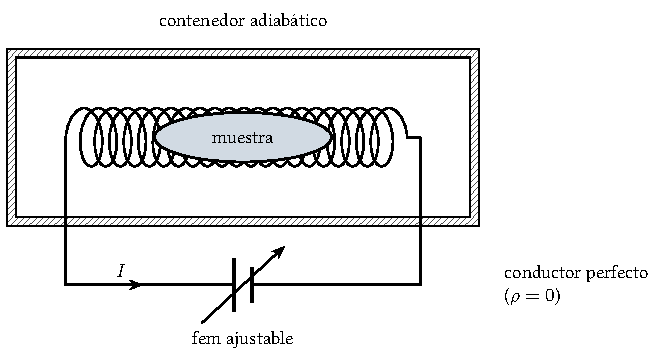
\includegraphics{figuras/solenoide.pdf}
\end{figure}
Sea un solenoide, el cual está construido por un conjunto de espiras hechas de un material tal que su
resistividad $\rho=0$ (es decir, el material es superconductor), el cual está conectado a una
batería con una fem (fuerza electromotriz) ajustable. El sistema termodinámico de interés se
encuentra dentro del solenoide y el solenoide se encuentra encerrado dentro de un contenedor
adiabático.

\begin{observacion}
  No olvidar que la fem es la energía que una fuente entrega por unidad de carga eléctrica para que
  estas puedan recorrer un circuito (y sí, no es una fuerza, sino una diferencia de potencial
  eléctrico).
\end{observacion}

Si no ocurren cambios en el sistema y si la corriente es constante, la batería no debe suministrar
fem, ya que el alambre es superconductor: por la relación $V=R\,I$, si $R=0$ entonces $V=0$, ya que
no hay disipación por una resistividad nula.

Sea $I$ la corriente y sea la magnetización local en el sistema $\vec{M}(\vec{r})$. La corriente $I$
se puede cambiar al modificar la fem en la batería; en consecuencia, la magnetización $\vec{M}(\vec{r})$
también cambia. Asumiendo que la magnetización en todo punto $\vec{r}$ es una función univaluada de
la corriente, es decir,
\begin{equation*}
  \vec{M}(\vec{r})=\vec{M}(\vec{r};I),
\end{equation*}
donde el punto y coma significa que $I$ es un parámetro de la magnetización, más que una variable
independiente.

Aquellos sistemas para los que $\vec{M}(\vec{r};I)$ no es una función univaluada, se dice que este
sistema exhibe una propiedad llamada \textbf{histéresis magnética}. Esta propiedad implica que, cuando
el campo externo se retira del sistema, queda una magnetización remanente. Esto es más común en los
sistemas ferromagnéticos (no como los paramagnéticos o diamagnéticos).

Este análisis es válido también para sistemas ferromagnéticos; en general, se consideran solo
materiales paramagnéticos, diamagnéticos o antiferromagnéticos.

Si el sistema termodinámico no está dentro del solenoide, la corriente $I$ produciría un campo
magnético (en realidad $\vec{H}$ es el campo magnético, $\vec{B}$ es llamado densidad de flujo
magnético) $\vec{B}_e(I)$. Este campo externo puede ser función de la posición dentro del solenoide,
pero es lineal en $I$:
\begin{equation*}
  \boxed{\vec{B}_e=\vec{b}\,I}
\end{equation*}
donde $\vec{b}$ es una función vectorial de la posición.

Si se incrementa la corriente, se incrementa $\vec{B}_e$ y el momento magnético cambia en respuesta.
Para que esto ocurra, la batería suministra trabajo, porque hay una relación entre el trabajo y los
cambios en $\vec{B}_e$ y $\vec{M}$. La tasa de cambio del trabajo hecho por la batería está dada por
\begin{equation*}
  \frac{\dbar W_{\mathrm{mag}}}{\dd t}=I\cdot(\text{voltaje}),
\end{equation*}
donde este voltaje denota la fem inducida por los cambios en las espiras.

La fem inducida tiene $2$ contribuciones:
\begin{enumerate}[label=\alph*),itemsep=2pt]
  \item La primera es independiente del sistema termodinámico y es el resultado del cambio en el
    flujo magnético asociado con $\vec{B}_e$. Es decir, para un solenoide vacío, porque el trabajo
    solo es el cambio en la energía del campo magnético:
    \begin{equation*}
      \dbar W_{\mathrm{mag}}=\dd\left[\frac{1}{2\mu_0}\int B_e^{2}\,\dd V\right],\qquad B_e^{2}=\vec{B}_e\cdot\vec{B}_e,
    \end{equation*}
    % NOTA: el manuscrito dice "flujo eléctrico asociado con B_e" y rotula la integral como "energía mag. promedio"; se escribió flujo magnético (el flujo asociado con B_e es magnético) y se dejó la expresión de la energía almacenada en el campo.
    donde la integral se toma sobre todo el solenoide (volumen) y
    $\mu_0=4\pi\times10^{-7}\ \mathrm{T\,m/A}$ es la permeabilidad magnética del vacío (qué tan fácil
    se magnetiza o induce el campo magnético).
  \item La segunda contribución es debida al sistema termodinámico; el cambio en el momento magnético
    infinitesimal de cada elemento del sistema contribuye de forma separada y aditiva a la fem
    inducida y, además, la fem cambia debido a la tasa de cambio en el momento y a su posición en el
    solenoide. Para determinar esta contribución, consideremos un modelo particular para un dipolo
    magnético (polo sur--norte) en $\vec{r}$: una pequeña espira de área $\vec{a}$ y corriente $i$, con
    momento magnético $\vec{m}=i\,\vec{a}$ (el dipolo más elemental).
    \begin{figure}[H]
      \centering
      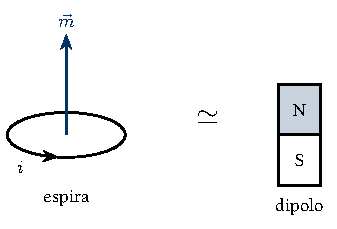
\includegraphics{figuras/dipolo.pdf}
    \end{figure}

    Si la corriente en el solenoide es $I$, el campo producido por el solenoide en $\vec{r}$ es
    $\vec{B}_e(\vec{r})=\vec{b}(\vec{r})\,I$ (como ya se dijo). Este campo inducido sobre la espira
    produce un flujo a través de la espira de corriente de magnitud $\vec{b}(\vec{r})\cdot\vec{a}\,I$;
    por lo que la inductancia (la resistencia a los cambios en la corriente eléctrica) es
    $\vec{b}(\vec{r})\cdot\vec{a}$. Por lo que, si la corriente en la espira cambia, se induce un
    voltaje en el solenoide dado por
    % NOTA: es la inductancia mutua entre la espira y el solenoide.
    \begin{equation*}
      \text{voltaje}=\bigl(\vec{b}(\vec{r})\cdot\vec{a}\bigr)\frac{\dd i}{\dd t}
      =\vec{b}(\vec{r})\cdot\frac{\dd\vec{m}}{\dd t}
      =\frac{1}{I}\,\vec{B}_e(\vec{r})\cdot\frac{\dd\vec{m}}{\dd t},
    \end{equation*}
    por lo que el trabajo hecho por la batería es
    \begin{equation*}
      \frac{\dbar W_{\mathrm{mag}}}{\dd t}=\vec{B}_e(\vec{r})\cdot\frac{\dd\vec{m}}{\dd t}.
    \end{equation*}
    A pesar de lo simple del modelo, se mantiene para cambios en el momento de los dipolos
    elementales. Si $\vec{M}(\vec{r})$ es la magnetización (momento dipolar magnético por unidad de
    volumen en el sistema en el punto $\vec{r}$), se tiene
    \begin{equation*}
      \vec{m}=\int\vec{M}(\vec{r})\,\dd V.
    \end{equation*}
    Por lo tanto, para obtener el trabajo total se suma sobre todos los dipolos elementales en todo
    el volumen,
    \begin{equation*}
      \frac{\dbar W_{\mathrm{mag}}}{\dd t}=\int\vec{B}_e\cdot\frac{\dd\vec{M}}{\dd t}\,\dd V.
    \end{equation*}
\end{enumerate}
Si se suman ambas contribuciones se tiene
\begin{equation*}
  \boxed{\dbar W_{\mathrm{mag}}=\dd\left[\frac{1}{2\mu_0}\int B_e^{2}\,\dd V\right]+\int\bigl(\vec{B}_e\cdot\dd\vec{M}\bigr)\,\dd V}
\end{equation*}
Este es el resultado fundamental en el que se construye la termodinámica del trabajo magnético.

De forma general, $\vec{M}(\vec{r})$ cambiará punto a punto dentro del sistema, incluso si $\vec{B}_e$
es constante (debido a inhomogeneidades inherentes o efectos de borde del sistema). Considerando en
nuestro caso solo materiales homogéneos con $\vec{B}_e$ constante y asumiendo que el sistema
termodinámico tiene forma elipsoidal (por simplicidad, ya que esta geometría permite manejar de
forma más simple la desmagnetización del sistema cuando $\vec{B}_e$ desaparece); para este tipo de
sistemas la magnetización $\vec{M}$ es independiente de la posición; por lo tanto,
\begin{equation*}
  \dbar W_{\mathrm{mag}}=\dd\left[\frac{1}{2\mu_0}\int B_e^{2}\,\dd V\right]+\vec{B}_e\cdot\dd\vec{\mathcal{I}},
  \qquad\vec{\mathcal{I}}=\int\vec{M}\,\dd V=\vec{M}V,
\end{equation*}
donde $\vec{\mathcal{I}}$ es el momento dipolar magnético total del sistema.

Por lo que, desde el punto de vista termodinámico, se tiene que los cambios en la energía son
\begin{align*}
  \dd(\text{Energía})&=T\,\dd S-P\,\dd V+\dbar W_{\mathrm{mag}}+\sum_{i=1}^{r}\mu_i\,\dd N_i\\
  &=T\,\dd S-P\,\dd V+\underbrace{\dd\left[\frac{1}{2\mu_0}\int B_e^{2}\,\dd V\right]}_{\text{energía del solenoide solo}}+\vec{B}_e\cdot\dd\vec{\mathcal{I}}+\sum_{i=1}^{r}\mu_i\,\dd N_i.
\end{align*}
Este término no es parte del sistema termodinámico, sino que se debe a la contribución a la energía
magnetostática del solenoide solo, por lo que es conveniente absorber este término en la energía
interna del sistema. Definiendo la energía como
\begin{equation*}
  U\equiv\text{Energía}-\frac{1}{2\mu_0}\int B_e^{2}\,\dd V,
\end{equation*}
donde $U$ es la energía total contenida en un solenoide, relativa al estado en el que el sistema es
removido y el solenoide se queda con su campo $\vec{B}_e$; entonces
\begin{equation*}
  \boxed{\dd U=T\,\dd S-P\,\dd V+B_e\,\dd\mathcal{I}_B+\sum_{i=1}^{r}\mu_i\,\dd N_i}
\end{equation*}
donde $\mathcal{I}_B$ es la componente del momento dipolar magnético paralela a $\vec{B}_e$.
% NOTA: el manuscrito dice "componente del momento dipolar eléctrico paralelo a B_e"; por el contexto es el momento dipolar magnético.

Por lo tanto, el parámetro extensivo que puede describir las propiedades magnéticas de un sistema es
$\mathcal{I}_B$, la componente del momento magnético total paralelo al campo externo. El parámetro
intensivo en la representación energética es $B_e$. Entonces
\begin{equation*}
  U=U(S,V,\mathcal{I}_B,N_1,\dots,N_r)\quad\text{es la relación fundamental}
\end{equation*}
y
\begin{equation*}
  B_e=\pdvc{U}{\mathcal{I}_B}{S,V,N_1,\dots,N_r}\quad\text{es la ecuación de estado.}
\end{equation*}

Para un caso más general de una muestra elipsoidal no coaxial con el campo magnético, \emph{no} es
posible considerar que la única contribución de $\vec{\mathcal{I}}$ al trabajo magnético sea la
paralela a $\vec{B}_e$, sino que se deben considerar las $3$ componentes (y si no es uniforme, se
vuelve un tensor de al menos $9$ componentes):
\begin{equation*}
  U=U(S,V,\mathcal{I}_x,\mathcal{I}_y,\mathcal{I}_z,N_1,\dots,N_r)\qquad\text{(en coordenadas cartesianas)},
\end{equation*}
con $[B_e]=\text{tesla}\ (\mathrm{T})$ y $[\mathcal{I}_B]=\text{joule/tesla}\ (\mathrm{J/T})$.

La relación de Euler para este sistema será
\begin{equation*}
  \boxed{U=TS-PV+B_e\mathcal{I}+\sum_{j=1}^{r}\mu_jN_j}
\end{equation*}
Notemos que la relación de Gibbs--Duhem es
\begin{equation*}
  \boxed{S\,\dd T-V\,\dd P+\mathcal{I}\,\dd B_e+\sum_{j=1}^{r}N_j\,\dd\mu_j=0}
\end{equation*}

Una característica importante de este tipo de sistemas surge al analizar las condiciones de
equilibrio, y es que no es posible imponer constricciones ante el momento magnético; en la práctica,
el momento magnético \emph{no puede ser constreñido}. Aunque el campo magnético sí puede ser
especificado y controlado y, por tanto, ajustar el valor del momento magnético, \emph{no hay paredes
restrictivas al momento magnético}. A pesar de lo anterior, la estructura de la termodinámica aún
puede ser aplicada y se mantiene a pesar de estos problemas.

Para cerrar este tema, veamos un ejemplo de la relación fundamental de un sistema paramagnético:
\begin{equation*}
  U=NRT_0\exp\left[\frac{S}{NR}+\frac{\mathcal{I}^{2}}{N^{2}\mathcal{I}_0^{2}}\right],
\end{equation*}
donde $T_0$ e $\mathcal{I}_0$ son constantes positivas. No describe un sistema en particular, pero es
un modelo simple para describir interacciones termomagnéticas.

\section{Capacidad calorífica y funciones de respuesta}

Ya hemos analizado la importancia física de las primeras derivadas de la relación fundamental. Las
segundas derivadas, por otra parte, describen propiedades materiales y usualmente son de mayor
interés físico que las primeras derivadas; este tipo de funciones es usualmente conocido como
\textbf{funciones de respuesta}, dado que usualmente representan la respuesta de los sistemas a
estímulos externos. Posteriormente regresaremos a la estructura fundamental de ellas y su relación;
sin embargo, por ahora veremos que el conjunto básico de segundas derivadas para sistemas no
magnéticos son solo tres; el resto están relacionadas entre sí.

\subsection*{Coeficiente de expansión térmica}

Se define como
\begin{equation*}
  \boxed{\alpha\equiv\frac{1}{v}\pdvc{v}{T}{P}}
\end{equation*}
o, en términos de las variables extensivas,
\begin{equation*}
  \alpha=\frac{N}{V}\pdvc{(V/N)}{T}{P,N}=\frac{1}{V}\pdvc{V}{T}{P}.
\end{equation*}
El coeficiente de expansión térmica es el incremento fraccional en el volumen, por incremento
unitario en la temperatura $T$, de un sistema mantenido a presión constante (y a número de moles
constante).

\subsection*{Compresibilidad isotérmica}

Se define como
\begin{equation*}
  \boxed{\kappa_T\equiv-\frac{1}{v}\pdvc{v}{P}{T}=-\frac{1}{V}\pdvc{V}{P}{T}}
\end{equation*}
Es el decremento fraccional en el volumen $V$ por incremento unitario en la presión, a temperatura
constante.

\subsection*{Capacidad calorífica molar a presión constante}

Las mayúsculas son sin molar ($C_P=Nc_P$). Se define como
\begin{equation*}
  \boxed{c_P\equiv T\pdvc{s}{T}{P}=\frac{T}{N}\pdvc{S}{T}{P}=\frac{1}{N}\left(\frac{\dbar Q}{\dd T}\right)_{P}}
\end{equation*}
Es el flujo cuasiestático de calor por mol requerido para producir un incremento unitario en la
temperatura de un sistema mantenido a presión constante.

Para sistemas con números de moles constantes, el resto de las segundas derivadas pueden expresarse
en términos de las $3$ previas ($\alpha$, $\kappa_T$, $c_P$). Posteriormente analizaremos por qué
ocurre esto, en términos de las llamadas \textbf{relaciones de Maxwell}.

Una de estas relaciones es
\begin{equation*}
  \pdvc{T}{V}{S,N}=-\pdvc{P}{S}{V,N},
\end{equation*}
la cual se sigue del teorema de Schwarz:
\begin{equation*}
  \pdv{V}\left(\pdv{U}{S}\right)=\pdv{S}\left(\pdv{U}{V}\right),
\end{equation*}
con $\pdvc{T}{V}{S,N}$ que representa el cambio de temperatura asociado con una expansión adiabática
del volumen. Notemos que $\pdvc{P}{S}{V,N}=T\left(\dfrac{\dd P}{\dbar Q}\right)_{V,N}$ es el producto
de la temperatura y el cambio de presión asociado con la introducción de un flujo de calor en el
sistema a volumen constante. Entonces, la relación entre ellas no es evidente, ya que parecen no
estar relacionadas.
% NOTA (manuscrito): al margen aparece "Ver f. exp." (ilegible/no resuelto).

El análogo a esta relación en la representación entrópica es
\begin{equation*}
  \pdvc{(1/T)}{V}{U,N}=\pdvc{(P/T)}{U}{V,N},
\end{equation*}
% NOTA: en el manuscrito el subíndice de la primera derivada aparece como "V,N"; la variable que se mantiene fija junto con N es U (para que ambos lados tengan las mismas variables independientes).
que usamos en el caso de van der Waals, a partir del teorema de Schwarz.

A partir de las diversas representaciones termodinámicas se pueden establecer relaciones entre
diversas segundas derivadas en términos del conjunto básico $c_P$, $\alpha$ y $\kappa_T$. Para
ilustrar lo anterior, se pueden introducir dos segundas derivadas adicionales.

\subsection*{Compresibilidad adiabática}

Se define como
\begin{equation*}
  \boxed{\kappa_S\equiv-\frac{1}{v}\pdvc{v}{P}{S}=-\frac{1}{V}\pdvc{V}{P}{S}}
\end{equation*}
Esta cantidad caracteriza la disminución del volumen asociada con un incremento isentrópico de la
presión (como en el caso de un sistema aislado adiabáticamente).

\subsection*{Capacidad calorífica molar a volumen constante}

Se define como
\begin{equation*}
  \boxed{c_v\equiv T\pdvc{s}{T}{v}=\frac{T}{N}\pdvc{S}{T}{V}=\frac{1}{N}\left(\frac{\dbar Q}{\dd T}\right)_{V}}
\end{equation*}
con $C_V=Nc_v$. % NOTA: el manuscrito escribe "C_V = N c_p"; por el contexto es C_V = N c_v.
Mide el flujo cuasiestático de calor por mol requerido para producir un incremento unitario en la
temperatura de un sistema mantenido a volumen constante.

\begin{proposicion}[Relaciones entre segundas derivadas]
  Se puede probar que
  \begin{align*}
    c_P&=c_v+\frac{Tv\alpha^{2}}{\kappa_T}\qquad\text{o}\qquad C_P=C_V+\frac{TV\alpha^{2}}{\kappa_T},\\
    \kappa_T&=\kappa_S+\frac{Tv\alpha^{2}}{c_P}\qquad\text{o}\qquad\kappa_T=\kappa_S+\frac{TV\alpha^{2}}{C_P}.
  \end{align*}
\end{proposicion}
% NOTA: el manuscrito escribe las formas molares como "c_P = c_v + TV\alpha^2/(N\kappa_T)" y "\kappa_T=\kappa_S+TV\alpha^2/(Nc_P)"; con v=V/N son las mismas expresiones. No se incluye demostración en el manuscrito.

\begin{ejercicio}
  Para un material particular, $c_P$, $\alpha$ y $\kappa_T$ son tabulados como función de $T$ y $P$.
  Encuentre el volumen molar como función de $T$ y $P$.
\end{ejercicio}

\begin{solucion}
  Como $c_P$, $\alpha$ y $\kappa_T$ son funciones de $T$ y $P$, y se busca $v$ como función de estas
  mismas variables, es decir, $v=v(T,P)$, nos conviene trabajar en el plano $T$--$P$, que es parte del
  ``espacio termodinámico'' donde existe $S=S(U,V,N)$ y las ecuaciones de estado.
  \begin{figure}[H]
    \centering
    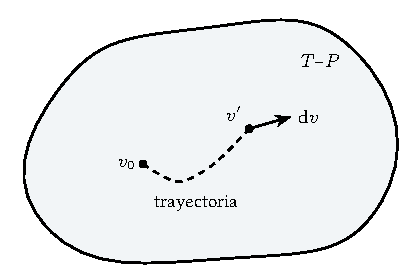
\includegraphics{figuras/region-TP.pdf}
  \end{figure}
  En este plano, $v=v(T,P)$, por lo que los desplazamientos en $v$ en una región dada del mismo son
  \begin{equation*}
    \dd v=\pdvc{v}{P}{T}\dd P+\pdvc{v}{T}{P}\dd T=(-v\kappa_T)\,\dd P+(v\alpha)\,\dd T,
  \end{equation*}
  sustituyendo las definiciones de $\kappa_T=-\frac{1}{v}\pdvc{v}{P}{T}$ y $\alpha=\frac{1}{v}\pdvc{v}{T}{P}$.
  De esta relación se puede factorizar $v$, de modo que
  \begin{equation*}
    \boxed{\frac{\dd v}{v}=-\kappa_T\,\dd P+\alpha\,\dd T}
  \end{equation*}
  Si tomamos como punto de referencia $(T_0,P_0)$ en el plano $T$--$P$ y se busca llegar hasta el punto
  $(T',P')$, se puede integrar por la trayectoria conveniente:
  \begin{equation*}
    \int_{v_0}^{v'}\frac{\dd v}{v}=\int_{T_0}^{T'}\alpha(T,P)\,\dd T-\int_{P_0}^{P'}\kappa_T(T,P)\,\dd P
    \quad\text{o bien}\quad
    \ln\frac{v'}{v_0}=\int_{T_0}^{T'}\alpha(T,P)\,\dd T-\int_{P_0}^{P'}\kappa_T(T,P)\,\dd P.
  \end{equation*}
  \begin{figure}[H]
    \centering
    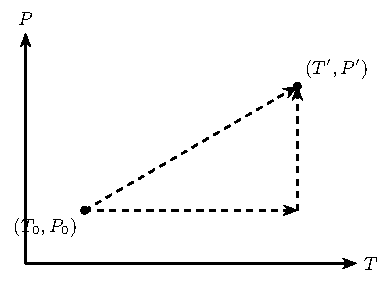
\includegraphics{figuras/camino-PT.pdf}
  \end{figure}
  Dependiendo de la trayectoria, $\dd P$ o $\dd T$ pueden anularse a trozos.
  % NOTA: como dv/v es un diferencial exacto (v es función de estado), la integral no depende de la trayectoria; se requiere que \alpha y \kappa_T sean compatibles (\partial\alpha/\partial P=-\partial\kappa_T/\partial T).
\end{solucion}

\begin{ejercicio}[3.9.3]
  Calcule el coeficiente de expansión $\alpha$ y la compresibilidad isotérmica $\kappa_T$ en términos
  de $P$ y $v$ para un sistema con ecuación de estado de van der Waals,
  \begin{equation*}
    P=\frac{RT}{v-b}-\frac{a}{v^{2}}.
  \end{equation*}
\end{ejercicio}

\begin{solucion}
  Ya que en este caso se piden $\alpha$ y $\kappa_T$ en el plano $P$--$v$, nos conviene partir de la
  ecuación de estado mecánica y deshacernos de $T$; despejando $T$,
  \begin{equation*}
    P+\frac{a}{v^{2}}=\frac{RT}{v-b}\qquad\text{o}\qquad T=\left(P+\frac{a}{v^{2}}\right)(v-b)\frac{1}{R},
  \end{equation*}
  de modo que los cambios en $T=T(P,v)$ son
  \begin{equation*}
    \dd T=\pdvc{T}{P}{v}\dd P+\pdvc{T}{v}{P}\dd v.
  \end{equation*}
  De acuerdo con la definición de las funciones de respuesta, $\alpha=\frac{1}{v}\pdvc{v}{T}{P}$;
  podemos obtenerlo del término $\pdvc{T}{v}{P}$:
  \begin{align*}
    \pdvc{T}{v}{P}&=\frac{1}{R}\left[\left(-\frac{2a}{v^{3}}\right)(v-b)+\left(P+\frac{a}{v^{2}}\right)(1)\right]
      =\frac{1}{R}\left[-\frac{2a}{v^{2}}+\frac{2ab}{v^{3}}+P+\frac{a}{v^{2}}\right]\\
    &=\frac{1}{R}\left[P-\frac{a}{v^{2}}+\frac{2ab}{v^{3}}\right]
     =\frac{1}{Rv^{3}}\left[Pv^{3}-av+2ab\right].
  \end{align*}
  Como $\pdvc{v}{T}{P}=\left[\pdvc{T}{v}{P}\right]^{-1}$,
  \begin{equation*}
    \pdvc{v}{T}{P}=\frac{Rv^{3}}{Pv^{3}-av+2ab},
    \qquad\text{y con }\alpha=\frac{1}{v}\pdvc{v}{T}{P}:\qquad
    \boxed{\alpha=\frac{Rv^{2}}{Pv^{3}-av+2ab}}
  \end{equation*}
  Ahora, para obtener $\kappa_T=-\frac{1}{v}\pdvc{v}{P}{T}$ nos conviene escribir $P=P(T,v)$, ya que
  $\dd P=\pdvc{P}{v}{T}\dd v+\pdvc{P}{T}{v}\dd T$ y obtener $\kappa_T$ a partir de la primera
  derivada. Entonces, con $P=\dfrac{RT}{v-b}-\dfrac{a}{v^{2}}$,
  \begin{equation*}
    \pdvc{P}{v}{T}=-\frac{RT}{(v-b)^{2}}+\frac{2a}{v^{3}},
  \end{equation*}
  y sustituyendo $RT=\left(P+\dfrac{a}{v^{2}}\right)(v-b)$,
  \begin{align*}
    \pdvc{P}{v}{T}&=-\frac{P+a/v^{2}}{v-b}+\frac{2a}{v^{3}}
      =\frac{1}{v-b}\left[-P-\frac{a}{v^{2}}+\frac{2a}{v^{3}}(v-b)\right]\\
    &=\frac{1}{v-b}\left[-P+\frac{a}{v^{2}}-\frac{2ab}{v^{3}}\right]
     =\frac{1}{v^{3}(v-b)}\left[-Pv^{3}+av-2ab\right].
  \end{align*}
  % NOTA: el manuscrito escribe "T=(P+v/a^2)(v-b)/R" (typo por a/v^2) y da el resultado final como "\kappa_T=v^3(v-b)/(P-av+2ab)". Rehaciendo la cuenta a partir de las líneas anteriores (que sí son correctas) se obtiene el resultado siguiente, en el que se conservan v^2 y P v^3 en el numerador/denominador; verificar contra el manuscrito.
  Como $\kappa_T=-\dfrac{1}{v}\left[\pdvc{P}{v}{T}\right]^{-1}$,
  \begin{equation*}
    \boxed{\kappa_T=\frac{v^{2}(v-b)}{Pv^{3}-av+2ab}}
  \end{equation*}
  Como comprobación, en el límite de gas ideal ($a\to0$, $b\to0$) se obtiene $\alpha=\dfrac{R}{Pv}=\dfrac{1}{T}$ y
  $\kappa_T=\dfrac{v^{3}}{Pv^{3}}=\dfrac{1}{P}$, que son los valores conocidos.
\end{solucion}

\begin{ejercicio}[3.9.5]
  De las ecuaciones $c_P=c_v+\dfrac{Tv\alpha^{2}}{\kappa_T}$ y $\kappa_T=\kappa_S+\dfrac{Tv\alpha^{2}}{c_P}$,
  demuestre que $\dfrac{c_P}{c_v}=\dfrac{\kappa_T}{\kappa_S}$.
\end{ejercicio}

\begin{solucion}
  De las ecuaciones dadas,
  \begin{equation*}
    c_P-c_v=\frac{Tv\alpha^{2}}{\kappa_T},\qquad\kappa_T-\kappa_S=\frac{Tv\alpha^{2}}{c_P},
  \end{equation*}
  por lo que, dividiendo,
  \begin{equation*}
    \frac{c_P-c_v}{\kappa_T-\kappa_S}=\frac{Tv\alpha^{2}/\kappa_T}{Tv\alpha^{2}/c_P}=\frac{c_P}{\kappa_T}.
  \end{equation*}
  Entonces
  \begin{equation*}
    c_P-c_v=\frac{c_P(\kappa_T-\kappa_S)}{\kappa_T}=c_P-\frac{c_P\kappa_S}{\kappa_T}
    \quad\Longrightarrow\quad
    c_v=\frac{c_P\kappa_S}{\kappa_T},
    \qquad\text{o bien}\qquad
    \boxed{\frac{c_v}{c_P}=\frac{\kappa_S}{\kappa_T}}
  \end{equation*}
  (la cantidad $Tv\alpha^{2}$ es no nula, de modo que el cociente anterior está bien definido cuando
  $\alpha\neq0$).
\end{solucion}

\begin{ejercicio}[3.9.6]
  Una relación fundamental simple que exhibe algunas de las propiedades cualitativas de los sólidos
  cristalinos típicos es
  \begin{equation*}
    u=A\,e^{b(v-v_0)^{2}}\,s^{4/3}\,e^{s/3R},
  \end{equation*}
  donde $A$, $b$ y $v_0$ son constantes positivas.
  \begin{enumerate}[label=\alph*),itemsep=2pt]
    \item Muestre que el sistema satisface el teorema de Nernst.
    \item Muestre que $c_v$ es proporcional a $T^{3}$ a temperaturas bajas (lo cual fue explicado por
      P.\ Debye en un análisis de mecánica estadística).
    \item Muestre que $c_v\to3R$ a temperaturas altas. Esto es llamado ``valor de equipartición'', que
      es observado y demostrado por Debye en el mismo análisis de mecánica estadística.
    \item Muestre que para $P=0$ el coeficiente de expansión térmica se anula para este modelo, lo que
      es incorrecto. Calcule el valor de $v$ a $P=0$.
  \end{enumerate}
\end{ejercicio}

\begin{solucion}
  \textbf{a)} Calculando primero $T$, con $T=\pdvc{u}{s}{v}$:
  \begin{align*}
    \pdvc{u}{s}{v}&=A\,e^{b(v-v_0)^{2}}\pdv{s}\left[s^{4/3}e^{s/3R}\right]
      =A\,e^{b(v-v_0)^{2}}\left[\frac{4}{3}s^{1/3}e^{s/3R}+s^{4/3}\left(\frac{1}{3R}e^{s/3R}\right)\right],\\
    &\boxed{T=A\,e^{b(v-v_0)^{2}}\left[\frac{4}{3}s^{1/3}+\frac{1}{3R}s^{4/3}\right]e^{s/3R}}
  \end{align*}
  De acuerdo con el postulado de Nernst, $T\to0$ si $s\to0$. Para $s\to0$ en $T$, notemos que
  $e^{s/3R}\to1$, mientras que entre $\frac{4}{3}s^{1/3}$ y $\frac{1}{3R}s^{4/3}$ el término que
  decrece más lento es $\frac{4}{3}s^{1/3}$; por lo tanto
  \begin{equation*}
    T\simeq\frac{4}{3}\,A\,e^{b(v-v_0)^{2}}\,s^{1/3}\qquad\text{cuando }s\to0.
  \end{equation*}
  % NOTA: el manuscrito escribe "e^{s/3R}\to0 muy rápido"; en realidad e^{s/3R}\to1 cuando s\to0 (lo que se anula es s^{1/3}). La conclusión no cambia.
  Asimismo,
  \begin{equation*}
    \lim_{s\to0}T=A\,e^{b(v-v_0)^{2}}\left[\frac{4}{3}s^{1/3}+\frac{1}{3R}s^{4/3}\right]e^{s/3R}\Bigg|_{s\to0}=0.
  \end{equation*}
  Por lo tanto se cumple el teorema de Nernst, y $T\to0$ (temperaturas bajas, cuando $s$ es pequeño).

  \textbf{b)} Ahora se debe calcular $c_v$, el cual está dado como $c_v=T\pdvc{s}{T}{v}$. Entonces se
  puede usar $\pdvc{T}{s}{v}$ e invertir la relación:
  \begin{align*}
    \pdvc{T}{s}{v}&=A\,e^{b(v-v_0)^{2}}\left\{\left[\frac{4}{9}s^{-2/3}+\frac{4}{9R}s^{1/3}\right]e^{s/3R}+\left[\frac{4}{3}s^{1/3}+\frac{1}{3R}s^{4/3}\right]\frac{1}{3R}e^{s/3R}\right\}\\
    &=A\,e^{b(v-v_0)^{2}}e^{s/3R}\left[\frac{4}{9}s^{-2/3}+\frac{4}{9R}s^{1/3}+\frac{4}{9R}s^{1/3}+\frac{1}{9R^{2}}s^{4/3}\right]\\
    &=A\,e^{b(v-v_0)^{2}}e^{s/3R}\left[\frac{4}{9}s^{-2/3}+\frac{8}{9R}s^{1/3}+\frac{1}{9R^{2}}s^{4/3}\right],
  \end{align*}
  por lo que
  \begin{equation*}
    c_v=T\pdvc{s}{T}{v}=\frac{T}{\pdvc{T}{s}{v}}
    =\frac{\dfrac{4}{3}s^{1/3}+\dfrac{1}{3R}s^{4/3}}{\dfrac{4}{9}s^{-2/3}+\dfrac{8}{9R}s^{1/3}+\dfrac{1}{9R^{2}}s^{4/3}}
  \end{equation*}
  (los factores $A\,e^{b(v-v_0)^{2}}e^{s/3R}$ se cancelan).
  Factorizando $s^{-2/3}$ en el numerador y en el denominador,
  \begin{equation*}
    \boxed{c_v=\frac{\dfrac{4}{3}s+\dfrac{1}{3R}s^{2}}{\dfrac{4}{9}+\dfrac{8}{9R}s+\dfrac{1}{9R^{2}}s^{2}}}
  \end{equation*}
  % NOTA: en el manuscrito el primer término del denominador aparece como "4/3"; al multiplicar (4/9)s^{-2/3} por s^{2/3} se obtiene 4/9, que es lo que se usa aquí (y lo que da c_v\simeq3s para s pequeño).
  Para probar que $c_v\propto T^{3}$ partimos de lo encontrado en el inciso anterior: si $s\to0$,
  $T\simeq C\,s^{1/3}$ con $C=\frac{4}{3}A\,e^{b(v-v_0)^{2}}$, por lo que $s\simeq(T/C)^{3}\propto T^{3}$.
  Asimismo, $c_v=T\pdvc{s}{T}{v}$, por lo que a $s\to0$
  \begin{equation*}
    c_v\simeq T\,\pdv{T}\left(\frac{T}{C}\right)^{3}=\frac{3T^{3}}{C^{3}}
    \quad\Longrightarrow\quad
    c_v\propto T^{3}\quad\text{cuando }s\to0\ \text{(temperaturas bajas)}.
  \end{equation*}
  Este resultado también se obtiene directamente de la expresión de $c_v$ anterior: para $s\to0$,
  $c_v\simeq\frac{4s/3}{4/9}=3s$.

  \textbf{c)} Para temperaturas altas, en $u=A\,e^{b(v-v_0)^{2}}s^{4/3}e^{s/3R}$ el término dominante es
  el que crece más rápido, es decir, $e^{s/3R}$, y
  $T=A\,e^{b(v-v_0)^{2}}\left[\frac{4}{3}s^{1/3}+\frac{1}{3R}s^{4/3}\right]e^{s/3R}$. Entonces
  $T\propto e^{s/3R}$ ($T\to\infty$) a orden dominante; tomando el logaritmo,
  $\ln T\propto\ln e^{s/3R}$, es decir, $\ln T\propto\dfrac{s}{3R}$ para $T$ grande, o $s\simeq3R\ln T$.
  Del cálculo de la capacidad calorífica $c_v=T\pdvc{s}{T}{v}$, para $T\to\infty$,
  \begin{equation*}
    c_v\simeq T\,\pdv{T}\left(3R\ln T\right)_v\simeq T\left(3R\cdot\frac{1}{T}\right)=3R.
  \end{equation*}
  Este resultado se confirma con la expresión exacta de $c_v$: para $s\to\infty$ dominan los términos
  en $s^{2}$, y $c_v\to\dfrac{s^{2}/(3R)}{s^{2}/(9R^{2})}=3R$. Pero $R$ es una constante que se usa por
  número de moles y $k_B$ es por partícula, con $R=N_Ak_B$; por lo tanto $c_v\to3k_B$ por partícula.

  \textbf{d)} Para este caso se debe calcular $P=-\pdvc{u}{v}{s}$:
  \begin{equation*}
    P=-A\,s^{4/3}e^{s/3R}\pdv{v}e^{b(v-v_0)^{2}}=-A\,s^{4/3}e^{s/3R}\left[2b(v-v_0)e^{b(v-v_0)^{2}}\right]
    =-2b(v-v_0)\left[A\,e^{b(v-v_0)^{2}}s^{4/3}e^{s/3R}\right],
  \end{equation*}
  es decir,
  \begin{equation*}
    P=-2b(v-v_0)\,u.
  \end{equation*}
  En este caso $P=0$ solo cuando $v=v_0$ (ya que $u>0$ para $s>0$). Como
  $\alpha=\frac{1}{v}\pdvc{v}{T}{P}$, en el caso donde $P=0$, $v=v_0$ es constante y
  $\pdvc{v}{T}{P}=0$, por lo que
  \begin{equation*}
    \boxed{\alpha=0}\qquad\text{y el volumen molar a }P=0\text{ es }v=v_0.
  \end{equation*}
  Lo anterior es incorrecto, ya que un sólido se expande con $T$.
\end{solucion}

\begin{ejercicio}[3.9.13]
  La susceptibilidad magnética isotérmica molar se define como
  \begin{equation*}
    \chi\equiv\frac{\mu_0}{N}\pdvc{\mathcal{I}}{B_e}{T}.
  \end{equation*}
  Muestre que esta susceptibilidad para el modelo paramagnético dado por la relación
  \begin{equation*}
    U=NRT_0\exp\left[\frac{S}{NR}+\frac{\mathcal{I}^{2}}{N^{2}\mathcal{I}_0^{2}}\right]
  \end{equation*}
  varía inversamente con la temperatura, y evalúe $\chi_1$, definida como el valor de $\chi$ para
  $T=1\ \mathrm{K}$.
\end{ejercicio}

\begin{solucion}
  Con $T=\pdvc{U}{S}{\mathcal{I},N}$ y $B_e=\pdvc{U}{\mathcal{I}}{S,N}$:
  \begin{align*}
    B_e&=NRT_0\left[\frac{2\mathcal{I}}{N^{2}\mathcal{I}_0^{2}}\right]\exp\left[\frac{S}{NR}+\frac{\mathcal{I}^{2}}{N^{2}\mathcal{I}_0^{2}}\right]
      =\frac{2RT_0\,\mathcal{I}}{N\mathcal{I}_0^{2}}\exp\left[\frac{S}{NR}+\frac{\mathcal{I}^{2}}{N^{2}\mathcal{I}_0^{2}}\right],\\
    T&=NRT_0\left[\frac{1}{NR}\right]\exp\left[\frac{S}{NR}+\frac{\mathcal{I}^{2}}{N^{2}\mathcal{I}_0^{2}}\right]
      =T_0\exp\left[\frac{S}{NR}+\frac{\mathcal{I}^{2}}{N^{2}\mathcal{I}_0^{2}}\right].
  \end{align*}
  Por lo que
  \begin{equation*}
    B_e=\frac{2R\,\mathcal{I}\,T}{N\mathcal{I}_0^{2}}
    \qquad\text{o}\qquad
    \mathcal{I}=\frac{N\mathcal{I}_0^{2}}{2RT}\,B_e,
  \end{equation*}
  es decir, $\mathcal{I}=\mathcal{I}(B_e,T)$. Entonces
  \begin{equation*}
    \chi=\frac{\mu_0}{N}\pdvc{\mathcal{I}}{B_e}{T}=\frac{\mu_0}{N}\pdv{B_e}\left(\frac{N\mathcal{I}_0^{2}}{2RT}B_e\right)
    =\frac{\mu_0\,\mathcal{I}_0^{2}}{2RT},
    \qquad\text{por lo que}\quad\boxed{\chi=\frac{\mu_0\mathcal{I}_0^{2}}{2RT}\propto\frac{1}{T}}
  \end{equation*}
  (ley de Curie). Asimismo,
  \begin{equation*}
    \boxed{\chi_1=\frac{\mu_0\mathcal{I}_0^{2}}{2R}}
  \end{equation*}
  % NOTA: el manuscrito escribe el momento magnético como "I_e" e "I_{e0}"; se usa \mathcal{I} e \mathcal{I}_0 por consistencia con las secciones anteriores.
\end{solucion}

\section{Transferencia de calor: conducción, convección y radiación}

% Pendiente: aún no está en las notas.

